\subsection{Dateien sichern}
Zu Beginn einer Datenanalyse sollte eine Momentaufnahme (Snapshot) des aktuellen Systems gespeichert werden. Dazu gehört ein Abbild des RAM- sowie des Festplattenspeichers.\\

\noindent\textbf{RAM Speicher sichern}\\
\noindent Bei einer ausführlicheren Systemanalyse sollte auch der RAM Speicher untersucht werden. Für Linux/Unix Systeme gibt es Programme, die ein Speicherabbild des RAM Speichers erstellen können (z.B. Memfetch). Für Windows gibt es keine solche Anwendungen. Jedoch kann über Umwege auf das Pagefile zugegriffen werden. Das Pagefile enthält die Speicherseiten die bei Swap-Operationen (vom RAM-Speicher werden Speicherseiten auf die Festplatte auslagert, um den Arbeitsspeicher zu entlasten) auf der Festplatte gespeichert werden. Um dies zu erreichen, muss das System über den Power-Button (nicht die konventionelle Methode über das Menü) ausschalten. Dadurch wird verhindert dass das PAgefile gelöscht wird. Um nun Zugriff auf dieses zu erhalten darf von der Festplatte nicht mehr gebootet werden, da dabei das PAgefile überschrieben werden würde. Um nun Zugriff auf die Datei zu erhalten, muss auf die Festplatte von einem anderen System zugegriffen werden (z.B. als Slave-Festplatte).Danach kann über verschiedene Tools auf die Datei zugegriffen werden. 
Ein anderer Weg, um Zugriff auf den RAM Speicher zu erhalten ist, einen STOP-Error herbeizuführen. Zuvor kann in den Erweiterten Systemeinstellungen (hängt vom verwendeten Betriebssystem ab) eingestellt werden, dass ein komplettes Speicherabbild erstellt werden soll (Abb. \ref{ram}).\\

\begin{figure}[h]
    \centering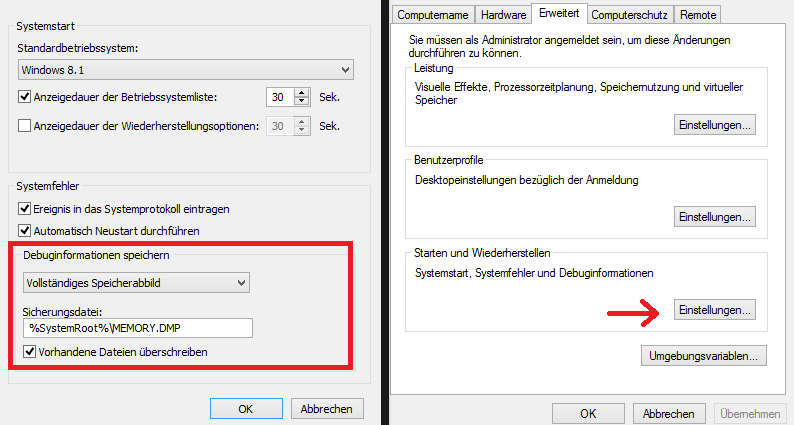
\includegraphics[scale=0.7]{Bilder/RAM.png}
  \caption{Einstellungen für RAM-Seicher Dmp-File}
  \label{ram}
\end{figure}

\noindent Ruft man nun einen STOP-Error herbei, so wird ein gesamtes Speicherabbild im angegeben Pfad gespeichert. Ein solchen Fehler absichtlich auszulösen kann über eine Tastenkombination, die zuvor in einem Registry Eintrag definiert wird, ausgelöst werden. Ein Beispiel dafür wäre:\\\\
\noindent\emph{HKEY\_LM \textbackslash System\textbackslash CurrentControlSet\textbackslash Services\textbackslash i8042prt\textbackslash ParamtersValue \newline Name: CrashOnCtrlScrollData Type: REG\_DWORDData:(1 = enabled)}\\\\
\noindent Nun kann durch das Halten der Strg-Taste und das zweimalige Tippen auf Rollen ein STOP-Error ausgelöst werden. Programme, mit denen man nun das Dmp-File bearbeiten kann werden von Windows selbst bereitgestellt.\\

\noindent\textbf{Speicherabbild des Festplattenspeichers}\\
\noindent Neben ein RAM-Speicherabbild wird bei einer ausführlichen Analyse ein Speicherabbild der Festplatte benötigt. Es gibt spezielle Anwendungen die ein komplettes Speicherabbild der Festplatte erstellen können. Als kommerzielle Lösung stellt Symantec Norton Ghost zur Verfügung. Um eine forensische Analyse durchzuführen werden meist jedoch speziellere Tools verwendet. Eine kostenlose Möglichkeit ein Festplattenabbild zu erstellen ist durch das dd Tool möglich. Dieses ist sowohl für Linux als auch für Windows verfügbar und kopiert Blockweise Speicher von einer Festplatte oder Partition auf einer andere. In Abb. \ref{fest} wird die komplette Partition f: auf d: als cdisk.img gespeichert.\\

\begin{figure}[h]
    \centering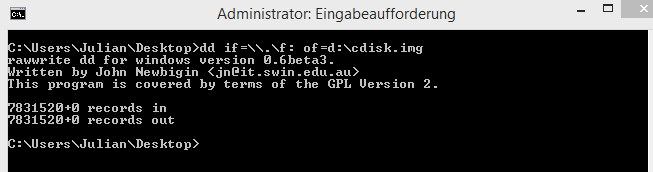
\includegraphics[scale=0.7]{Bilder/DD.png}
  \caption{Erstellung eines Speicherabbilds mit dd}
  \label{dd}
\end{figure}

\noindent Neben dieser vereinfachten Methode gibt es noch weitere Möglichkeiten über kommerzielle Software, die für den Zweck einer forensischen Analyse entwickelt wurden, ein professionelles Festplattenabbild zu erstellen. Zu diesen gehören:
\begin{itemize}
\item EnCase
\item Winhex
\item ProDiscover
\item SafeBack
\end{itemize}

\noindent Nachdem alle relevanten Daten gesichert wurden kann der Netzverkehr überprüft werden.